\section{Grappa}

Irregular applications are characterized by having unpredictable data-dependent access patterns and poor spatial and temporal locality. Applications in this class, including data mining, graph analytics, and various learning algorithms, are becoming increasingly prevalent in high-performance computing. These programs typically perform many fine-grained accesses to disparate sources of data, which is a problem even at multicore scales, but is further exacerbated on distributed memory machines.
It is often the case that naively porting an application to a PGAS system results in excessive communication and poor access patterns~\cite{pgas-analysis}, but this class of applications defies typical optimization techniques such as data partitioning, shadow objects, and bulk-synchronous communication transformations.
Luckily, applications in this class have another thing in common: abundant amounts of data access parallelism. This parallelism can be exploited in a number of different ways to improve overall throughput of these applications.

% The goal of the Grappa runtime is to provide a PGAS implementation that has been designed from the ground up to leverage massive amounts of parallelism to achieve high performance on irregular applications.

Grappa is a global-view PGAS runtime for commodity clusters which has been designed from the ground up to achieve high performance on irregular applications. The key is latency tolerance--long-latency operations such as reads of remote memory can be tolerated by switching to another concurrent thread of execution. Given abundant concurrency, there are opportunities to increase throughput by sacrificing latency. In particular, throughput of random accesses to remote memory can be improved by delaying communication requests and aggregating them into larger packets.

Highly tuned implementations of irregular applications in shared-memory, PGAS and message-passing paradigms, typically end up implementing similar constructs. Grappa includes these as part of its core infrastructure and simply asks the programmer to express concurrency which it can leverage to provide performance.

Grappa's programming interface, implemented as a C++11 library, provides high-level operations to access and synchronize through global shared memory, task spawning capabilities and parallel loop constructs for expressing concurrency. In addition, the Grappa ``standard library'' includes functions to manipulate a global heap, stock remote synchronization operations such as \emph{compare-and-swap}, and several synchronized global data structures. The following sections will explain the execution model of Grappa and the current C++ programming interface.

\begin{figure}[t]
  \centering
  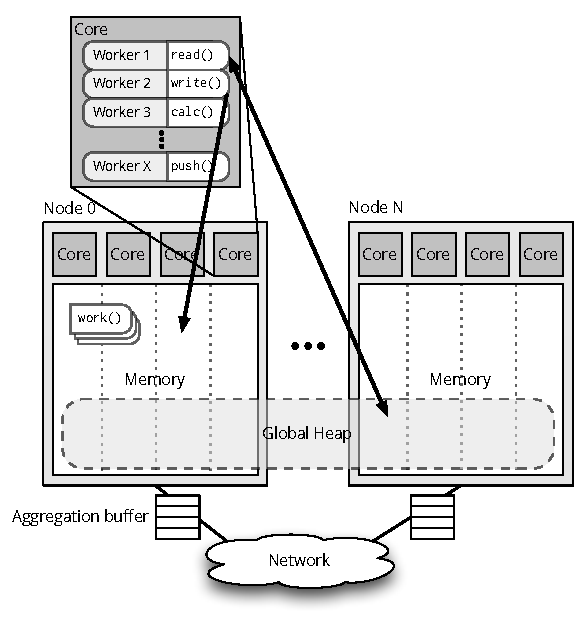
\includegraphics[width=0.5\textwidth]{figs/grappa_system.pdf}
  \caption{\emph{Grappa System Overview:}
    Thousands of workers are multiplexed onto each core, context switching to tolerate the additional latency of aggregating remote operations. Each core has exclusive access to a slice of the global heap which is partitioned across all nodes, as well as core-private data and worker stacks. Tasks can be spawned and executed anywhere, but are bound to a worker in order to be executed.
  }
  \label{fig:system}
\end{figure}

\subsection{Tasks and Workers}
Grappa uses a task-parallel programming model to make it easy to express concurrency.
A \emph{task} is simply a function object with some state and a function to execute.
Tasks may block on remote accesses or synchronization operations.
The Grappa runtime has a lightweight threading system that uses prefetching to scale up to thousands of threads on a single core with minimal increase in context-switch time.
In the runtime, \emph{Worker} threads pull these programmer-specified tasks from a queue and execute them to completion. When a task blocks, the worker thread executing it is simply suspended and consumes no computational resources until woken again by some event.

\subsection{Aggregated Communication}
The most basic unit of communication in Grappa is an \emph{active message}~\cite{vonEicken92}.
To make efficient use of the networks in high-performance systems, which typically achieve maximum bandwidth only for messages on the order of 64 KB, all communication in Grappa is sent via an aggregation layer that automatically buffers messages to the same destination.
% Communication in Grappa is achieved via \emph{active messages}~\cite{vonEicken92} in conjunction with bulk remote direct memory access (RDMA) operations. Various components of Grappa's runtime contribute different kinds of messages to move and modify remote data, perform synchronization, or spawn tasks. To make efficient use of the networks in high-performance systems, which perform better with larger messages (typically 64 KB), all communication in Grappa is sent through an aggregation layer that automatically accumulates messages to the same destination. When enough messages are ready to go to a particular destination node, they are serialized into a buffer and sent using RDMA.

\subsection{Global Memory}
In the PGAS style, Grappa has a notion of a global address space which is partitioned across the physical memories of the nodes in a cluster. Each core owns a portion of memory, which is divided among execution stacks for the core's Workers, a core-local heap, and a slice of the global heap.

All of these can be addressed by any core in the system using a \texttt{GlobalAddress}, which encodes both the owning core and the address on that core. Additionally, addresses into the global heap are partitioned in a block-cyclic fashion, so that a large allocation is automatically distributed among many nodes. For irregular applications, this helps avoid hot spots and is typically sufficient for random access.

All accesses to memory owned by another core must be done by that core via a message, even enforcing strict isolation between processes on the same physical memory. At the programming level, however, this is hidden behind higher-level remote operations, which in Grappa are called \emph{delegates}. Figure~\ref{fig:system} shows an example of a delegate \texttt{read} which blocks the calling task and sends a message to the owner, who sends a reply with the data and wakes the caller.

